\begin{figure*}[!ht]
	\centering{
		\hspace*{\fill}
\begin{subfigure}{0.43\textwidth}
   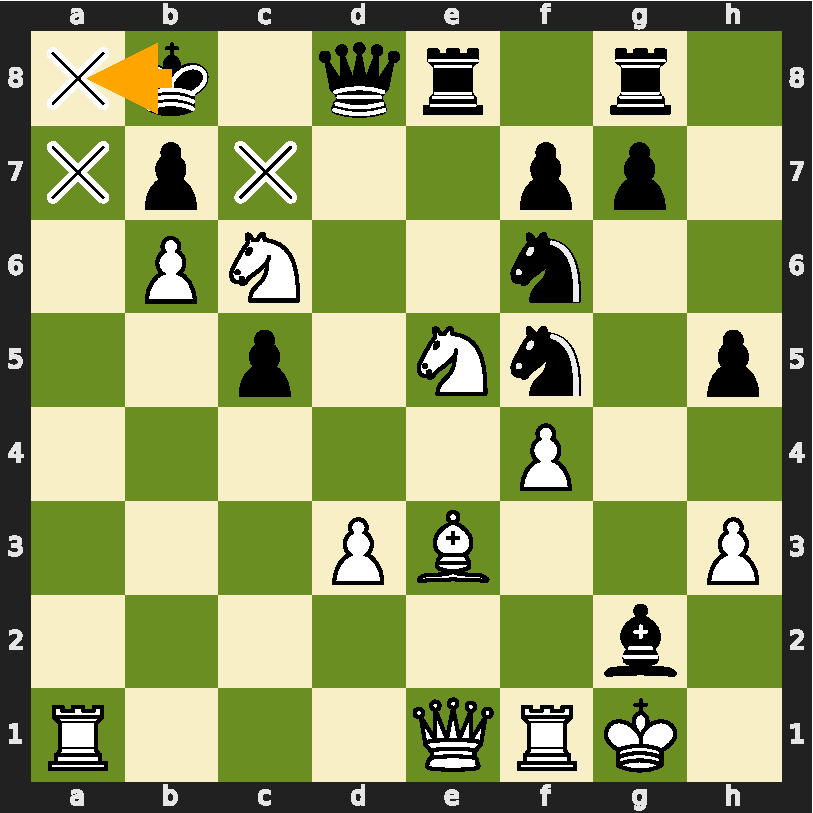
\includegraphics[width=\linewidth]{figures/board_check_king.pdf}
   \caption{\emph{Check + King}: Black king is in check and the predicted ending square is already covered by the white rook on \pos{a1}.} 
   \label{fig:error_check_king}
\end{subfigure}
\hspace*{\fill}
\begin{subfigure}{0.43\textwidth}
	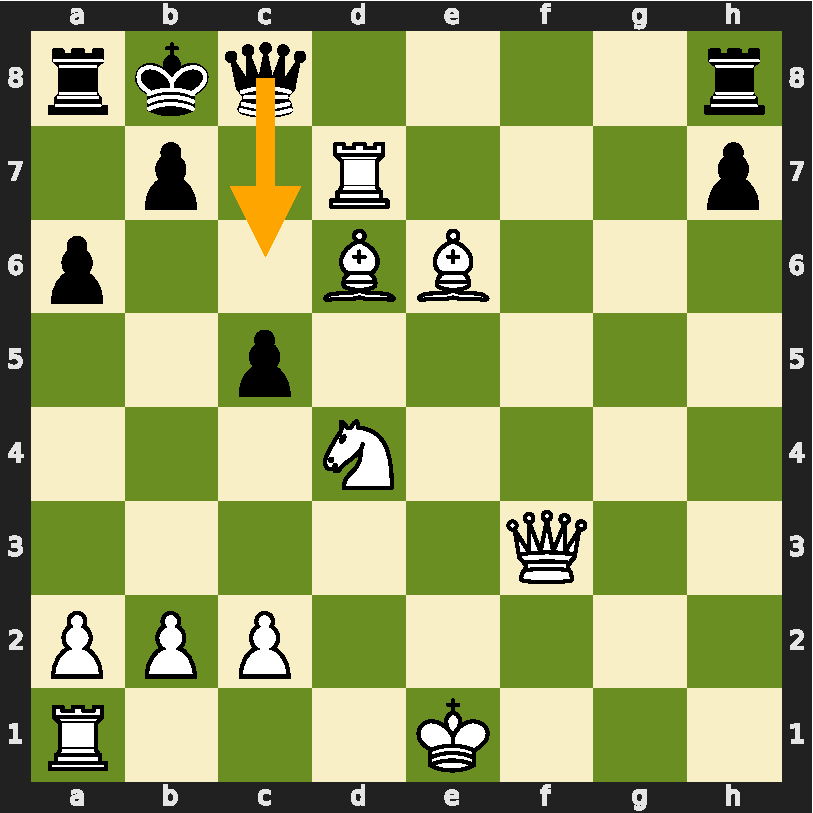
\includegraphics[width=\linewidth]{figures/board_check_no_king.pdf}
	\caption{\emph{Check + Other}: Black king is in check and the only legal move for the black queen is \pos{c7} but the model predicts \pos{c6}.} 
	\label{fig:error_check_no_king}
\end{subfigure}
\hspace*{\fill}
\\[1em]
\hspace*{\fill}
\begin{subfigure}{0.43\textwidth}
   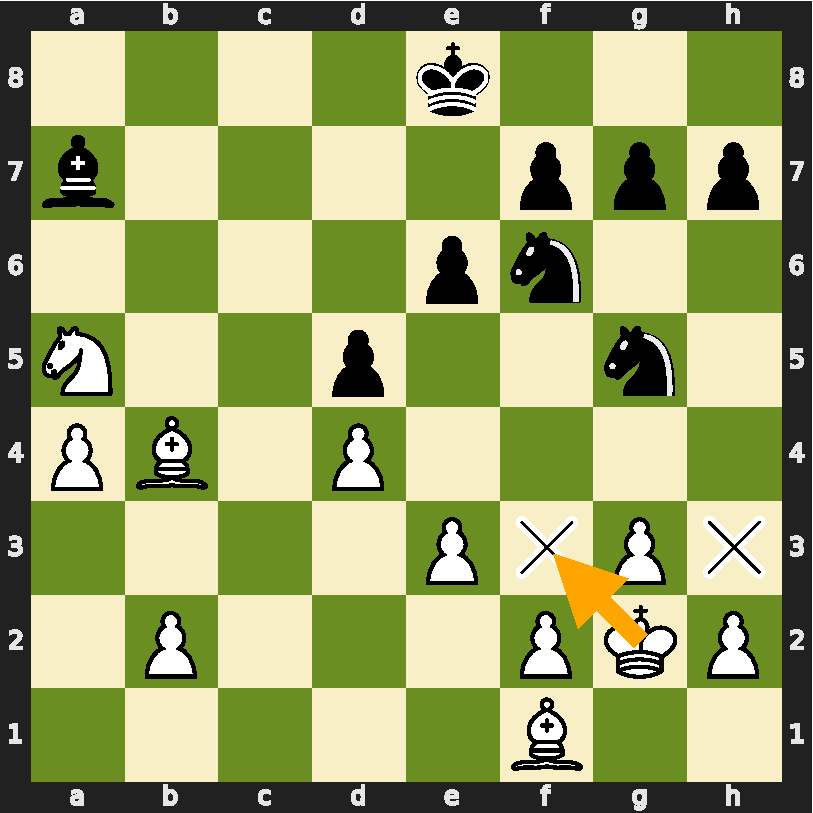
\includegraphics[width=\linewidth]{figures/board_no_check_king.pdf}
   \caption{\emph{No Check + King}: The predicted ending square \pos{f3} for the white king is guarded by the black knight at \pos{g5}.} 
   \label{fig:error_no_check_king}
\end{subfigure}
\hspace*{\fill}
\begin{subfigure}{0.43\textwidth}
	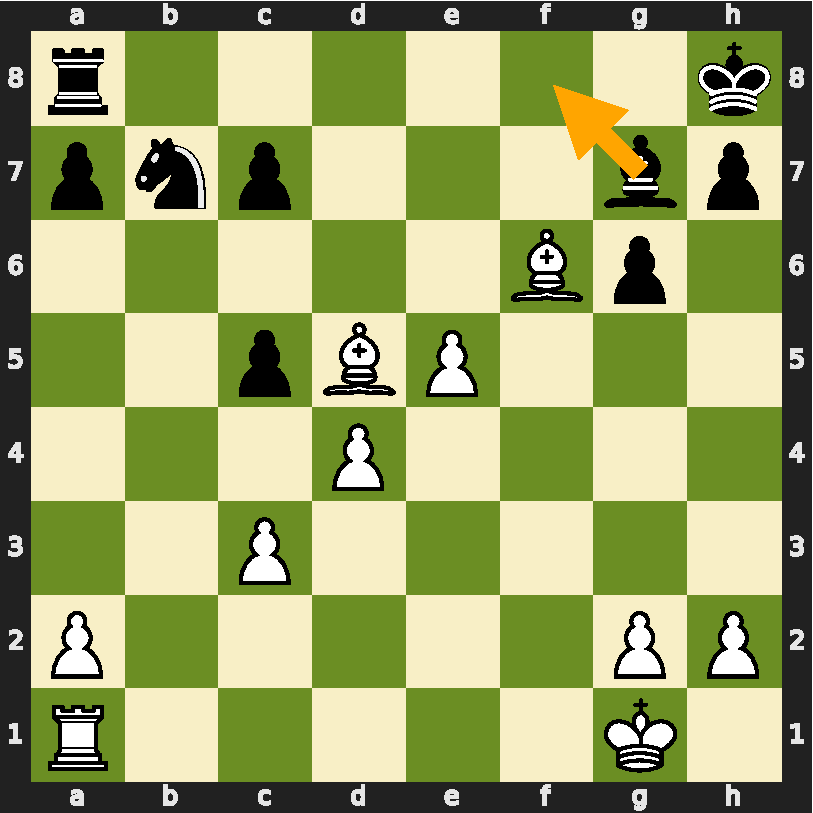
\includegraphics[width=\linewidth]{figures/board_no_check_no_king.pdf}
	\caption{\emph{No Check + Other}: The predicted ending square \pos{f8} for the black bishop exposes its king to the white bishop at \pos{f6}. } 
	\label{fig:error_no_check_no_king}
\end{subfigure}
\hspace*{\fill}
\caption{Four combinations of the king being in check or not, and if the king is moved or not, that can result in Pseudo Legal errors.}
\label{fig:pseudo_legal_errors}
}
\end{figure*}



